\documentclass[10pt]{article}

\usepackage[margin=1in]{geometry}
\usepackage{amsmath}
\usepackage{amssymb}
\usepackage{graphicx}
\usepackage{booktabs}
\usepackage{algorithm}
\usepackage{algpseudocode}
\usepackage[hidelinks]{hyperref}
\usepackage{cleveref}

% ---------------------------------------------------------------------------
% Editing notes
% - The method's name is set in one place: \methodname below.
% - Claim-type labels are the five macros below. Every claim in the main text
%   carries one; claims.md lists each claim with its source.
% - "% source:" comments give the generated result file each number comes
%   from (paths relative to the repository root).
% ---------------------------------------------------------------------------
% Compact lists (no extra package needed).
\makeatletter
\def\@listi{\leftmargin\leftmargini \topsep 3pt plus 1pt \parsep 0pt \itemsep 1pt plus 1pt}
\let\@listI\@listi
\def\@listii{\leftmargin\leftmarginii \topsep 1pt \parsep 0pt \itemsep 0pt}
\makeatother

% Let floats share pages with text.
\renewcommand{\topfraction}{0.9}
\renewcommand{\bottomfraction}{0.8}
\renewcommand{\textfraction}{0.07}
\renewcommand{\floatpagefraction}{0.75}
\setcounter{topnumber}{3}
\setcounter{totalnumber}{4}

\newcommand{\methodname}{BC-NE}
\newcommand{\BN}{\methodname{}+BN}

\newcommand{\cpub}{\textit{\small (published)}}
\newcommand{\cder}{\textit{\small (our derivation)}}
\newcommand{\cpre}{\textit{\small (pre-registered)}}
\newcommand{\cdesc}{\textit{\small (descriptive)}}
\newcommand{\cinterp}{\textit{\small (interpretation)}}
\newcommand{\todo}[1]{\textbf{[TODO: #1]}}

\newcommand{\T}{^{T}}
\newcommand{\R}{\mathbb{R}}
\newcommand{\E}{\mathbb{E}}
\newcommand{\xiB}{\xi_{B}}

\title{Background-contrastive neighbor embedding:\\ method, evidence and open questions}
\author{Cassia Bastress}
\date{October 2026}

\begin{document}
\maketitle

% =====================================================================
\section{Summary}
\label{sec:summary}

\paragraph{The method.} \methodname{} embeds a target dataset $X_T$ in two dimensions while suppressing variation it shares with a background dataset $X_B$. It builds the $k$-nearest-neighbor (kNN) graph of the targets not on the raw features but on \emph{local background residuals}. For each target point it finds its nearest background points and subtracts their mean and their top few principal directions; the kNN graph is then built on what remains. The graph is embedded with two-stage Neg-t-SNE, a negative-sampling neighbor embedding \cite{damrich2023tsne}. Optionally, the embedding also adds \emph{background negatives}: extra repulsion between target points whose background neighborhoods overlap. The two variants are written \methodname{} and \BN{}.

\paragraph{Key findings.}
\begin{enumerate}
  \item \textbf{The residual graph is what makes the method work.} On MNIST-on-grass (MNIST digits overlaid on grass photographs), \BN{} beats the earlier version of the method, which used the raw kNN graph with background negatives, on every confirmation seed: digit kNN accuracy 0.973 vs 0.931, a lead of $+0.036$ to $+0.046$ per seed \cpre. Without any background negatives, switching to the residual graph raises plain Neg-t-SNE by $+0.10$ to $+0.13$ \cdesc.
  % source: results/bsgraph/tables_phase2.md, results/bsgraph/comparisons.json
  \item \textbf{Background negatives are redundant once the graph is background-suppressed.} \BN{} vs \methodname{} on MNIST-on-grass: $+0.0014$, $0.0000$ and $+0.0020$ per seed, which is not consistent \cpre.
  % source: results/bsgraph/comparisons.json
  \item \textbf{On MNIST-on-grass the method ties cPCA$\to$t-SNE and is more stable across seeds.} \BN{} vs contrastive PCA followed by t-SNE: $+0.032$, $-0.006$, $+0.028$, not consistent \cpre. Across seeds, \BN{} ranges over 0.972--0.974 and cPCA$\to$t-SNE over 0.941--0.979 \cdesc.
  % source: results/bsgraph/tables_phase2.md
  \item \textbf{Global cPCA wins when the background is additive.} When target $=$ signal $+$ independent background, the target-minus-background covariance equals the signal covariance (\cref{sec:theory}) \cder. On three additive synthetic benchmarks, cPCA$\to$Neg-t-SNE beats raw-graph background negatives at every level \cdesc; on MNIST-on-grass, cPCA$\to$t-SNE beats them on every seed \cpre.
  \item \textbf{A local, cluster-then-cPCA pipeline beats raw-graph background negatives on two benchmarks built to defeat global projections.} Its within-cluster signal accuracy is 0.984--0.992, against 0.914 \cpre.
  % source: results/phase5b/tables_cyclic_local_cpca.md, results/phase5b/tables_between_local_cpca.md
  \item \textbf{On one of those benchmarks, raw-graph background negatives beat every global linear pipeline, including label-chosen ones}: 0.914 vs 0.530 for the best cPCA variant \cpre{} and 0.624 for the best labeled linear projection \cdesc.
  % source: results/phase5b/tables_cyclic.md
\end{enumerate}

\paragraph{Main open question.} The residual graph has been tested only on MNIST-on-grass, where the background is additive and global cPCA already does about as well. Its intended advantage, suppressing a background that no single global projection can remove, is untested: on non-additive real data, and on the synthetic benchmarks where global cPCA fails (\cref{sec:gaps}).

\paragraph{How claims are labeled.} Every claim carries one of five labels:
\begin{itemize}
  \item \cpub{}: a cited published result;
  \item \cder{}: our own derivation;
  \item \cpre{}: an experimental verdict under a rule committed before the results;
  \item \cdesc{}: a measurement with no verdict attached;
  \item \cinterp{}: our explanation, not directly tested.
\end{itemize}

% =====================================================================
\section{Problem setup and notation}
\label{sec:setup}

We have a \emph{target} dataset $X_T \in \R^{n_T\times D}$ and a \emph{background} dataset $X_B \in \R^{n_B\times D}$ in the same feature space. $X_B$ contains only nuisance variation, while $X_T$ contains the same kind of nuisance variation plus a target-specific \emph{signal}. The goal is a two-dimensional embedding $Y \in \R^{n_T\times 2}$ of the targets whose neighborhoods reflect the signal, not the background. This is the neighbor-embedding analogue of contrastive PCA (cPCA) \cite{abid2018cpca}, which finds directions with high target variance and low background variance.

\paragraph{Notation.}
\begin{itemize}
  \item $y_i \in \R^2$ is the embedding of target point $i$, and $d_{ij} = \|y_i - y_j\|$.
  \item $\phi(d) = 1/(1+d^2)$ is the Cauchy kernel, and $q_{ij} = \phi(d_{ij})$ is the model similarity.
  \item $p_{ij}$ is the data distribution over pairs: uniform over the directed edges of the symmetrized kNN graph of the targets, with $k = 15$ neighbors.
  \item $\xi$ is a noise distribution over pairs. $m$ is the number of uniform negatives per edge, and $m_B$ the number of background negatives per edge.
  \item $k_{\mathrm{loc}}$ is the number of background neighbors used for the residual, and $r$ the number of local background directions removed.
  \item $C_T$ and $C_B$ are the covariance matrices of $X_T$ and $X_B$; $\alpha \ge 0$ is cPCA's contrast parameter. $Q\T$ denotes the transpose of $Q$.
  \item \emph{Seeds.} Every dataset in this report is generated from a seed, and the same seed drives every random choice in the runs on it. \emph{Selection seeds} are used to choose settings; fresh \emph{confirmation seeds} are used for verdicts.
\end{itemize}

% =====================================================================
\section{Background: neighbor embeddings as contrastive learning}
\label{sec:background}

\paragraph{Attraction and repulsion.} t-SNE \cite{vandermaaten2008tsne} and UMAP \cite{mcinnes2018umap} can both be written as attraction along kNN edges plus repulsion between other pairs. t-SNE's repulsion comes from normalizing $q$ over all pairs; UMAP's comes from sampled noise pairs \cpub{} \cite{damrich2023tsne}. How the two forces are balanced places a method on an attraction--repulsion spectrum that runs from t-SNE-like to UMAP-like embeddings \cpub{} \cite{bohm2022spectrum}.

\paragraph{NCE vs negative sampling.} Damrich et al.\ \cite{damrich2023tsne} make this precise through contrastive learning. Both methods below sample positive pairs from $p$ and noise pairs from $\xi$, and train a classifier to tell them apart.
\begin{itemize}
  \item \textbf{Noise-contrastive estimation (NCE).} The classifier is $q_\theta/(q_\theta + m\xi)$, so the noise probability enters it. At the optimum $q_\theta = p$, whatever the (full-support) noise distribution $\xi$ \cpub{} (\cite{gutmann2010nce}; Theorem~1 of \cite{damrich2023tsne}).
  \item \textbf{Negative sampling.} The classifier is $q_\theta/(q_\theta + 1)$: the noise probability does \emph{not} enter it \cite{mikolov2013word2vec,levy2014neural}. Corollary~2 of \cite{damrich2023tsne} generalizes NCE to a model that learns $\bar Z p$ for a fixed $\bar Z$. With uniform noise over the $|X|$ pairs, negative sampling equals that generalized NCE with $\bar Z = |X|/m$, so it learns $q = (|X|/m)\,p$, a rescaled $p$ \cpub.
\end{itemize}
Neg-t-SNE is negative sampling with the Cauchy kernel. In the \texttt{contrastive-ne} package, its classifier is $q/(q+c)$ for a constant $c$ (default $c = 1$). Moving $c$ moves the embedding along the attraction--repulsion spectrum \cpub{} \cite{damrich2023tsne}.

\paragraph{Our extension: a general noise distribution.} Corollary~2 is stated for uniform $\xi$. Since background negatives make $\xi$ non-uniform, we need the optimum for a general $\xi$ \cder. The expected negative-sampling loss with classifier $q/(q+c)$ is
\begin{equation}
  \mathcal{L}(q) = \sum_{x} \Big[ -p(x)\log\frac{q(x)}{q(x)+c} \;-\; m\,\xi(x)\log\frac{c}{q(x)+c} \Big],
\end{equation}
summed over pairs $x = (i,j)$. Treat each $q(x)$ as a free variable. Setting the derivative to zero,
\begin{equation}
  -\frac{p}{q} + \frac{p + m\xi}{q + c} = 0
  \quad\Longrightarrow\quad
  q^*(x) = \frac{c\,p(x)}{m\,\xi(x)} .
  \label{eq:qstar}
\end{equation}
For $p(x) > 0$ the loss tends to $+\infty$ as $q \to 0$ and as $q \to \infty$, so this stationary point is the minimum. With uniform $\xi = 1/|X|$ and $c = 1$, \cref{eq:qstar} gives $q^* = (|X|/m)p$, recovering Corollary~2.

With background negatives, each edge with head $i$ draws $m$ uniform negatives and $m_B$ negatives from $\xiB(i,\cdot)$, the latter weighted by $\gamma$ in the loss. The expected noise weight on a pair is then $m\,\xi_U(i,j) + \gamma\, m_B\, \tilde\xi_B(i,j)$, where $\tilde\xi_B(i,j) = p_i\,\xiB(i,j)$ and $p_i$ is the head marginal of $p$. The same calculation gives
\begin{equation}
  q^*_{ij} = \frac{c\,p_{ij}}{m\,\xi_U(i,j) + \gamma\, m_B\, \tilde\xi_B(i,j)} .
  \label{eq:qstar-bg}
\end{equation}
Pairs that the background explains (large $\tilde\xi_B$) get a smaller target similarity, i.e.\ more repulsion. This includes kNN edges whose endpoints are close for background reasons.

The derivation is idealized. It rests on four assumptions:
\begin{itemize}
  \item each $q_{ij}$ can be set freely; a 2-D embedding cannot do this exactly;
  \item expectations replace sampling;
  \item the package's in-batch uniform negatives are treated as uniform over pairs;
  \item the package's clamping of the classifier output to $[10^{-4},1]$ is ignored.
\end{itemize}

\paragraph{UMAP.} The loss UMAP actually optimizes differs from the one stated in its paper; it has far less repulsion \cpub{} \cite{damrich2021umap}. Lemma~3 of \cite{damrich2023tsne} shows that UMAP's loss is negative sampling with the model $1/d_{ij}^2$ instead of the Cauchy kernel. The repulsive term of $1/d^2$ diverges as $d \to 0$, while Neg-t-SNE's stays bounded \cpub.

\paragraph{Initialization.} We initialize from the first two principal components, scaled so the first has standard deviation 1, as recommended for preserving global structure \cpub{} \cite{kobak2021init,damrich2023tsne}.

% =====================================================================
\section{The method}
\label{sec:method}

\subsection{Background-suppressed (residual) neighbor graph}
\label{sec:residual}

For each target point $x_i$:
\begin{enumerate}
  \item Find its $k_{\mathrm{loc}}$ nearest background points $N_B(i) \subset X_B$ (exact Euclidean search).
  \item Compute their mean $\mu_i$, and the top $r$ right singular vectors $V_i \in \R^{D\times r}$ of the centered neighbors $\{b - \mu_i : b \in N_B(i)\}$.
  \item Form the residual
  \begin{equation}
    \tilde x_i = (I - V_i V_i\T)(x_i - \mu_i).
    \label{eq:residual}
  \end{equation}
\end{enumerate}
The attraction graph is the exact $k = 15$ nearest-neighbor graph of the residuals $\{\tilde x_i\}$, symmetrized by union, with binary weights.

\begin{itemize}
  \item \textbf{Defaults:} $k_{\mathrm{loc}} = 30$, $r = 2$. They were selected on one dataset; the selection barely mattered (\cref{sec:dec-defaults}).
  \item \textbf{Properties:} the residual is invariant to sign flips of the columns of $V_i$. It needs no clustering of the background and no global projection.
  \item \textbf{What changes and what doesn't:} only the graph changes. The initialization and the background negatives (if used) are computed on the raw features.
\end{itemize}
% source: method/residual_graph.py; results/bsgraph/preregistration_phase2.md

\subsection{Two-stage Neg-t-SNE}

Neg-t-SNE \cite{damrich2023tsne} as implemented in \texttt{contrastive-ne} v0.4.0, non-parametric, with package defaults:
\begin{itemize}
  \item $m = 5$ negatives per edge, drawn from the current minibatch;
  \item $c = 1$;
  \item minibatches of $2^{15}$ directed edges;
  \item SGD with learning rate 1, annealed linearly to 0;
  \item elementwise gradient clipping at $\pm4$.
\end{itemize}

The schedule has two separate fits on the same graph:
\begin{itemize}
  \item \textbf{Stage 1:} 250 epochs from the PCA initialization.
  \item \textbf{Stage 2:} 500 epochs starting exactly from the Stage~1 embedding, with a fresh learning-rate annealing.
\end{itemize}
Background negatives, when used, are active in Stage~2 only.

\subsection{Optional background negatives}
\label{sec:xib}

$\xiB$ is a distribution over target pairs that look similar for background reasons.
\begin{enumerate}
  \item For each target point $i$, find its $k_B = 15$ nearest background points $N_B(i)$.
  \item Score target pairs by the Jaccard overlap $s_B(i,j) = |N_B(i)\cap N_B(j)|/|N_B(i)\cup N_B(j)|$.
  \item Keep the top $L = 30$ partners per point. All partners tied with the 30th are kept, up to $2L$; ties beyond that cap are broken by a seeded random draw, never by target distance.
  \item Set $\xiB(i,\cdot) \propto s_B(i,\cdot)$. Target kNN edges are not excluded.
\end{enumerate}

For each kNN edge with head $i$, Stage~2 adds $m_B$ negatives $b \sim \xiB(i,\cdot)$ with the loss term
\begin{equation}
  -\gamma \sum_{b=1}^{m_B} \log\Big(1 - \frac{\phi_{ib}}{\phi_{ib}+c}\Big), \qquad \gamma = 1.
\end{equation}
It uses the same $c$, kernel and clamping as the package's own negatives. A unit test checks that one background negative and one uniform negative at the same distance contribute identical loss and gradient.

By \cref{eq:qstar-bg}, this lowers the target similarity of pairs with overlapping background neighborhoods \cder. In words, the embedding learns roughly ``target similarity divided by background similarity'' \cinterp.

\begin{algorithm}[t]
\caption{\methodname{} (with optional background negatives)}
\label{alg:method}
\begin{algorithmic}[1]
\Require targets $X_T$, background $X_B$; $k_{\mathrm{loc}}=30$, $r=2$, $k=15$; optional $m_B$
\For{each target $x_i$}
  \State $N_B(i) \gets$ the $k_{\mathrm{loc}}$ nearest rows of $X_B$ to $x_i$
  \State $\mu_i \gets$ mean of $N_B(i)$;\; $V_i \gets$ top-$r$ right singular vectors of $N_B(i) - \mu_i$
  \State $\tilde x_i \gets (I - V_iV_i\T)(x_i - \mu_i)$
\EndFor
\State $G \gets$ exact $k$-NN graph of $\{\tilde x_i\}$, union-symmetrized, binary
\State $Y_0 \gets$ first two principal components of $X_T$, scaled so the first has std 1
\State $Y_1 \gets$ Neg-t-SNE$(G$, init $Y_0$, 250 epochs$)$
\If{$m_B > 0$}
  \State build $\xiB$ from Jaccard overlaps of the $k_B$-nearest background sets (raw features)
\EndIf
\State $Y \gets$ Neg-t-SNE$(G$, init $Y_1$, 500 epochs, plus $m_B$ negatives per edge from $\xiB$ if $m_B>0)$
\State \Return $Y$
\end{algorithmic}
\end{algorithm}

\subsection{Implementation}

\begin{itemize}
  \item \textbf{Package change:} the code adds an 11-line hook to the vendored package so that the trainer can add a term to each batch loss.
  \item \textbf{Exact graphs:} all kNN graphs are exact and built once per dataset. The package's own approximate graph is unseeded, so it is never used.
  \item \textbf{Determinism:} every fit runs with deterministic algorithms and seeded generators. The background sampler has its own generator, so turning it off reproduces the unmodified package bit for bit.
  \item \textbf{Checks:} reruns were checked to be bit-identical in every experiment.
\end{itemize}

% =====================================================================
\section{Design decisions and their evidence}
\label{sec:decisions}

Each subsection states what was chosen, the alternatives, and the evidence. The experiments are described in \cref{sec:evidence}.

\subsection{Neg-t-SNE rather than UMAP or t-SNE}
\label{sec:dec-neg}

\begin{itemize}
  \item \textbf{Choice and reason.} Negative sampling leaves the noise distribution out of its classifier, so changing $\xi$ changes the optimum (\cref{eq:qstar}) \cder. Under NCE the optimum is $p$ for any $\xi$ \cpub, and t-SNE has no noise distribution to change. The package was checked to use a single constant $c$, not $\xi$, in its classifier \cdesc.
  \item \textbf{Alternative rejected: UMAP.} Its effective $1/d^2$ model has a repulsion that diverges at short range \cpub{} \cite{damrich2023tsne}. That is exactly where background negatives act: on pairs that start close together because they share a background \cinterp.
  \item \textbf{Trade-off.} Without the background term, Neg-t-SNE was \emph{below} t-SNE on MNIST-on-grass: 0.858 vs 0.884, and vs 0.891 for PCA$\to$t-SNE \cdesc. Comparisons with t-SNE-based controls therefore also change the embedding algorithm (\cref{sec:gaps}).
  % source: results/mnist_grass/tables.md
\end{itemize}

\subsection{Putting the background into the noise distribution}
\label{sec:dec-noise}

\begin{itemize}
  \item \textbf{Choice.} The first version of the method changed only the repulsion: background negatives on top of the raw kNN graph. Under NCE this lever does not exist, because the noise distribution cancels at the optimum \cpub.
  \item \textbf{Evidence that it acts.} On three additive synthetic benchmarks (\cref{sec:synthetic}), raw-graph background negatives beat the best \emph{uniform extra negatives} control (the same number of extra negatives, drawn uniformly) on every confirmation seed \cpre. The gains in signal kNN accuracy over that control were:

  \begin{center}
  \begin{tabular}{lc}
    \toprule
    background type & gain over best uniform control \\
    \midrule
    orthogonal & $+0.51$ \\
    overlapping & $+0.18$ \\
    nonlinear & $+0.44$ \\
    \bottomrule
  \end{tabular}
  \end{center}
  % source: results/phase4/tables.md (pre-registered comparisons, confirmation seeds)

  They also beat a reference run moved toward the t-SNE end of the spectrum at every level \cpre.
  \item \textbf{The uniform control is weak} \cdesc. The background forms 6 equal, well-separated clusters, so about 5 in 6 uniform negatives land in another cluster, which is already far away. They add little force within a cluster. Beating this control shows that the repulsion has to be targeted; it does not show that $\xiB$'s targeting is the only kind that works. \Cref{sec:dec-jaccard} uses a stronger control.
\end{itemize}

\subsection{Background similarity from shared background neighbors}
\label{sec:dec-jaccard}

\begin{itemize}
  \item \textbf{$\xiB$ pairs share the background, not the signal} \cdesc.
  \begin{itemize}
    \item Synthetic data: pairs share the true background cluster 100\% of the time. Their excess of same-signal pairs over chance is at most $+0.064$.
    % source: results/phase2/xi_b_diagnostics.csv; results/phase4/summary_medium_confirmation.json
    \item MNIST-on-grass: the same-digit excess is $+0.055$ to $+0.074$. The grass patches of $\xiB$ pairs are 3.8--4.0 apart, against 7.9--8.1 for random pairs.
    % source: results/mnist_grass/prechecks.md
  \end{itemize}
  \item \textbf{It beats a same-cluster oracle} \cpre. This control draws the extra negatives uniformly from the head's \emph{true} background cluster, a deliberate use of labels. $\xiB$ beats it:
  \begin{itemize}
    \item on the interaction benchmark: $+0.39$ signal kNN accuracy;
    \item on both subspace-conflict benchmarks (cyclic and between-cluster): $+0.21$ and $+0.22$ within-cluster signal accuracy.
  \end{itemize}
  So $\xiB$'s fine-grained neighborhoods matter, not just knowing the cluster \cinterp.
  % source: results/phase5a/tables_J.md; results/phase5b/tables_cyclic.md; results/phase5b/tables_between.md
  \item \textbf{Caveat} \cdesc. On the subspace-conflict benchmarks, the oracle was selected at the top of its grid ($m_B = 80$), and its selection-seed mean was still rising slowly (by $+0.01$ to $+0.02$ from $m_B = 40$ to 80). Its best possible value is unknown.
\end{itemize}

\subsection{The two-stage schedule}

\begin{itemize}
  \item \textbf{Why two separate fits.} The package's built-in early-exaggeration phase does nothing at its negative-sampling defaults, and it does not reset the learning rate \cdesc. Two separate fits give an exact handoff: Stage~2 starts from the Stage~1 embedding bit for bit, and is reproducible.
  \item \textbf{Not tested.} No single-stage ablation was run. The original reason for the warm-up was to let a global layout form before the background term acts, to avoid fragmentation. That is a design rationale, not a tested result \cinterp.
\end{itemize}

\subsection{Moving the background into the graph}
\label{sec:dec-graph}

Background negatives change only the repulsion; the attraction still follows the raw kNN graph. Several measurements pointed to the raw graph as a limit \cdesc:
\begin{itemize}
  \item On both subspace-conflict benchmarks, raw-graph background negatives reach about the signal accuracy of the high-dimensional data itself: within-cluster accuracy 0.91, against 0.915--0.924 on the confirmation seeds.
  % source: results/phase5b/tables_cyclic.md, tables_between.md (detectability column)
  \item When the signal is weak in the graph itself (the weak-signal stress sets), the gains are small or absent.
  % source: results/phase4/stress/tables_stress.md
  \item In the additive benchmarks, 0 of about 925{,}000 kNN edges join different background clusters, so attraction can never pull the clusters together.
  % source: results/phase4/data_geometry.md (0 of 313574 + 312002 + 300033)
  \item On MNIST-on-grass, 44\% of a target's raw-graph neighbors are also among its 15 nearest images by grass patch.
  % source: results/bsgraph/phase1.md (raw grass recall 0.439)
\end{itemize}

\textbf{Counterexample} \cdesc. On MNIST-on-grass, raw-graph background negatives reached a digit accuracy of 0.931, above the raw graph's own digit accuracy on the same confirmation seeds (0.901; 0.903--0.905 on the selection seeds). So the ``graph ceiling'' is not strict \cinterp.
% source: results/mnist_grass/tables.md; results/bsgraph/phase1.md; results/mnist_grass/prechecks.md

\textbf{The main evidence} is the residual-graph result itself: \BN{} beats raw-graph background negatives on every MNIST-on-grass confirmation seed \cpre.

\subsection{A local residual graph rather than a global cPCA graph}
\label{sec:dec-local}

The alternative considered was a graph built on the top 10 global cPCA components. On MNIST-on-grass it was cleaner \cdesc:

\begin{center}
\small
\begin{tabular}{llcc}
  \toprule
  seeds & graph & graph digit accuracy & graph grass recall \\
  \midrule
  selection (0--2) & global cPCA-10 & 0.970 & 0.006 \\
  selection (0--2) & residual ($k_{\mathrm{loc}}=30$, $r=2$) & 0.962 & 0.056 \\
  confirmation (3--5) & global cPCA-10 & 0.957 & 0.006 \\
  confirmation (3--5) & residual ($k_{\mathrm{loc}}=30$, $r=2$) & 0.962 & 0.057 \\
  \bottomrule
\end{tabular}
\end{center}
% source: results/bsgraph/phase1.md

On the confirmation seeds the accuracy order reverses, but cPCA-10 keeps the much lower grass recall. On additive data, then, the local graph has no clear advantage. Its case rests on backgrounds that are not additive, where no single global projection removes them; that is untested (\cref{sec:gaps}) \cinterp.

\subsection{Defaults $k_{\mathrm{loc}} = 30$ and $r = 2$}
\label{sec:dec-defaults}

\begin{itemize}
  \item \textbf{The gate} \cpre. A graph-quality gate was committed before any residual graph was computed. On each selection seed, the selected variant had to beat the better of the raw-pixel and PCA-50 graphs by at least 0.02 in graph digit accuracy. It did, by $+0.025$, $+0.027$ and $+0.029$.
  \item \textbf{The choice of variant barely matters} \cdesc. All 15 variants on the grid ($k_{\mathrm{loc}} \in \{15,30,100\}$, $r \in \{0,1,2,5,10\}$) reach mean graph digit accuracy 0.954--0.964 on the selection seeds (0.951--0.965 per seed). Each is above both reference graphs: raw 0.904 and PCA-50 0.935. Even $r = 0$, which only subtracts the local background mean, clears both.
  \item \textbf{So a fixed, label-free default is supported} \cinterp, though only on this one dataset. The selection used labels, but it decided little.
\end{itemize}
% source: results/bsgraph/phase1.md

\subsection{Current status of background negatives}

\begin{itemize}
  \item \textbf{Redundant on MNIST-on-grass with the residual graph} \cpre. The smallest value on the grid, $m_B = 1$, was selected, and accuracy fell slowly as $m_B$ grew, from 0.973 at $m_B=1$ to 0.968 at $m_B=40$ \cdesc.
  % source: results/bsgraph/tables_phase2.md (appendix)
  \item \textbf{Untested elsewhere.} They have not been tested with the residual graph on any other data.
  \item \textbf{Why they may be redundant} \cinterp. The residual graph and $\xiB$ use the same information, each target's nearest background points: $\xiB$ uses it for repulsion, the residual graph for neighborhood definition. On this dataset, using it in the graph is what helps.
\end{itemize}

% =====================================================================
\section{When linear suppression works: theoretical observations}
\label{sec:theory}

\subsection{The population identity behind cPCA}
\label{sec:identity}

\paragraph{Claim} \cder, a standard argument. Suppose target $x_T = s + g + \varepsilon$ and background $x_B = g' + \varepsilon'$, where:
\begin{itemize}
  \item $s$, $g$ and $\varepsilon$ are independent;
  \item $g'$ has the same distribution as $g$;
  \item the noises have equal covariance $\sigma^2 I$.
\end{itemize}
Then $C_T - C_B = C_S$, the signal covariance.

\paragraph{Proof.} By independence the cross-covariances vanish, so $C_T = C_S + C_G + \sigma^2 I$ and $C_B = C_G + \sigma^2 I$. $\square$

\paragraph{Consequences.}
\begin{itemize}
  \item The identity holds for \emph{any} map producing $g$, linear or not: only $g$'s covariance enters, and it cancels.
  \item At $\alpha = 1$, cPCA's top directions are the signal's own directions. Only finite-sample error remains.
  \item For $\alpha > 1$, $C_T - \alpha C_B = C_S - (\alpha-1)(C_G + \sigma^2 I)$, so the signal survives in directions where the background has little variance \cder.
\end{itemize}

\paragraph{Breaking independence is not enough.} Suppose each background cluster has its own signal map, with zero mean and outside the span of the background. The cross-covariances still vanish and the identity survives, with a higher-dimensional $C_S$ \cder. A benchmark built this way was stopped at calibration: cPCA$\to$Neg-t-SNE already reached within-cluster signal accuracy 0.970--0.980 on its selection seeds \cdesc.
% source: results/phase5a/k_calibration.md

\subsection{Finding vs cleaning}
\label{sec:finding}

\paragraph{Claim} \cder. Let $P$ be the orthogonal projection onto the subspace spanned by the $k$ cPCA directions that are kept. Under the assumptions of \cref{sec:identity},
\begin{equation}
  \operatorname{Cov}(P x_T) = P C_S P + P C_G P + \sigma^2 P .
\end{equation}
The identity guarantees that cPCA \emph{finds} the signal directions. The projected data are \emph{clean} only if $C_G$ has no variance in the chosen subspace; otherwise the term $P C_G P$ remains, and the embedding still sees that background variation.

\paragraph{Illustration} \cdesc: the between-cluster benchmark (\cref{sec:synthetic}). There the signal lies inside the between-cluster span $U$, and the within-cluster nuisance lies in a separate block $V$.
\begin{itemize}
  \item For $\alpha < 1$, $C_T - \alpha C_B = C_S + (1-\alpha)(C_G + \sigma^2 I)$, so the top directions are $U$, then $V$.
  \item With $k \le 5$ components, cPCA keeps only $U$ and reveals the signal: within-cluster accuracy 0.989.
  \item At $k = 10$, the components also include $V$, and accuracy drops to 0.35. Embedding the labeled projection onto $U \cup V$ gives the same 0.34--0.36.
\end{itemize}
% source: results/phase5b/tables_between.md (cPCA variants by alpha and k); results/phase5b/runs_between_confirmation.csv (lin_U+V)
The between-cluster offsets that remain in $U$ do not affect within-cluster accuracy, which is computed inside each background cluster.

\subsection{Global vs local background variance}

\paragraph{Where a local method can help} \cinterp. A local method can beat a global projection where the background varies strongly \emph{globally} along the signal's directions, but weakly within a neighborhood.

\paragraph{What decides it} \cdesc. What decides whether cPCA fails is the fraction of signal variance lying \emph{outside} the directions of high global background variance, not the ratio of global to local background variance itself.
\begin{itemize}
  \item On an interaction benchmark, the ratio reached 46--69. But it was driven by a 2--10\% tilt of the signal into the background's span.
  \item At least 87\% of the signal variance lay outside that span on every seed, and cPCA used it.
\end{itemize}
% source: results/phase5a/data_diagnostics.md

\subsection{The cyclic construction}
\label{sec:cyclic-theory}

In the cyclic benchmark (\cref{sec:synthetic}) there are six background clusters with a 3-dimensional subspace $Q_k$ each. Within cluster $k$, the signal lies in $Q_k$ and the background nuisance in $Q_{k+1}$ (indices mod 6), with nuisance standard deviation $\sigma_w = \sqrt{5/3}$ and signal scale $\rho = 0.2$.

\paragraph{Block-aligned projections} \cder. Consider projections onto a union of whole blocks. Revealing cluster $k$ cleanly requires keeping $Q_k$ and dropping $Q_{k+1}$. Keeping $Q_k$ therefore prevents a clean reveal of cluster $k-1$, whose nuisance is $Q_k$. Around the cycle of six, at most every other cluster can be revealed cleanly: 3 of 6.

\paragraph{General projections} \cinterp, not proven. Let $a_k$ be the fraction of $Q_k$ kept by a general projection. Revealing cluster $k$ needs $\rho^2 a_k \gg \sigma_w^2 a_{k+1}$. Revealing two adjacent clusters would need $a_k$ to fall by more than $(\sigma_w/\rho)^2 \approx 42$ per step, which the isotropic noise floor limits. We do not state this as a theorem.

\paragraph{Observed} \cdesc. The best of the 64 labeled block subsets reveals exactly 3 clusters, with within-cluster accuracy 0.624. The best cPCA variants, which are not block-aligned, reach 0.530 on average (0.551 on the best seed).
% source: results/phase5b/tables_cyclic.md; results/phase5b/calibration.md

\paragraph{Why per-cluster cPCA still solves it} \cder. Within cluster $k$, $C^{(k)}_T - \alpha C^{(k)}_B = \rho^2 Q_k \Sigma_s Q_k\T - (\alpha-1)(\sigma_w^2 Q_{k+1}Q_{k+1}\T + \sigma^2 I)$, where $\Sigma_s$ is the covariance of the signal latent. For any $\alpha \ge 1$ the top directions lie in $Q_k$. A different projection is used in each cluster, so the cyclic conflict disappears. In the experiment, every per-cluster label-free $\alpha$ was above 1 (1.7 to 58.8) \cdesc, and local cPCA reached within-cluster accuracy 0.984--0.992 \cpre.

\subsection{The residual graph in these terms}
\label{sec:residual-theory}

\cinterp, untested. The residual in \cref{eq:residual} acts locally. The local mean removes the cluster centroid, and the top-$r$ local directions remove the local nuisance. In the cyclic benchmark each cluster's nuisance is 3-dimensional, so the default $r = 2$ removes only 2 of its 3 directions. On MNIST-on-grass, $r = 5$ was nearly identical to $r = 2$ (graph digit accuracy 0.961 vs 0.962 at $k_{\mathrm{loc}} = 30$) \cdesc.
% source: results/bsgraph/phase1.md

% =====================================================================
\section{Empirical evidence}
\label{sec:evidence}

\subsection{Evaluation protocol}
\label{sec:protocol}

\paragraph{Ground truth and pre-registration.}
\begin{itemize}
  \item Synthetic benchmarks have known signal and background labels; labels are used only to evaluate.
  \item Every experiment's settings, comparisons and decision rules were committed to the repository before the results they govern (\cref{app:repro}).
\end{itemize}

\paragraph{Seeds.} Each experiment chooses its settings (e.g.\ $m_B$) on selection seeds 0--2. Verdicts use fresh confirmation seeds, usually 3--5.

\paragraph{The verdict rule.} Runs are paired by seed. ``X beats Y, consistent across 3 paired seeds'' means the mean difference is positive \emph{and} every per-seed difference is positive. No $p$-values are reported. A comparison that fails this rule is reported as ``not consistent''.

\paragraph{Validity and checks.}
\begin{itemize}
  \item A synthetic dataset counts only if plain Neg-t-SNE hides its signal (signal kNN accuracy $\le 0.50$) but shows its background (background accuracy $\ge 0.90$), while the clean signal is separable (oracle accuracy $\ge 0.95$).
  \item One confirmation seed failed this check and was replaced under a rule added before any other result on that level.
  \item Rerun determinism was checked (bit-identical) in every experiment.
  \item Runs were flagged for collapse or fragmentation; none was flagged.
\end{itemize}

\paragraph{Metrics.} All are computed on the 2-D embedding.
\begin{itemize}
  \item \emph{Signal kNN accuracy}: a 15-nearest-neighbor classifier predicting the signal label, with stratified 5-fold cross-validation.
  \item \emph{Within-cluster signal accuracy}: the same, computed inside each true background cluster, size-weighted.
  \item \emph{Detectability}: within-cluster accuracy computed on the high-dimensional data.
  \item \emph{Recall vs grass}: the fraction of a point's 15 embedding neighbors that are also among its 15 nearest images by grass patch. Lower is better.
\end{itemize}

\paragraph{Controls and what each rules out.}
\begin{center}
\small
\begin{tabular}{ll}
  \toprule
  control & rules out \\
  \midrule
  plain Neg-t-SNE & (baseline) \\
  uniform extra negatives & the gain is just more repulsion \\
  t-SNE-end spectrum reference ($\bar Z = 100n$, $c = 500/n$) & the gain is a shift along the spectrum \\
  same-cluster oracle negatives & knowing the background cluster suffices \\
  cPCA$\to$Neg-t-SNE / UMAP / t-SNE & linear background suppression suffices \\
  t-SNE, PCA$\to$t-SNE & standard practice suffices \\
  \bottomrule
\end{tabular}
\end{center}
% source: spectrum reference constants from the package (Zbar = 100 n at s = 0; c = m Zbar / n^2)

\paragraph{Platforms.} The synthetic experiments ran on a laptop CPU, and MNIST-on-grass on the McGill Mathematics Slurm cluster (CPU only). No comparison mixes the two platforms. On a benchmark rerun, the two platforms differed by at most 0.027 in within-cluster accuracy, below every verdict margin \cdesc.
% source: results/mnist_grass/validation (Phase B table in results/mnist_grass/tables.md)

\subsection{Synthetic benchmarks}
\label{sec:synthetic}

All synthetic results below used the \textbf{raw} kNN graph with background negatives, the method's earlier form. The residual graph has not been tested on them.

\paragraph{The benchmarks.} All have $n_T = n_B = 5000$ points in $D = 50$ dimensions, noise std 0.1, and six equal-weight background clusters (simplex centers 30 apart in a 5-D latent space). The signal has four groups (simplex edge 6 in a 3-D latent space), scaled by $\rho$.
\begin{itemize}
  \item \textbf{Additive}: $x_T = \rho A z_s + B(z_b) + \varepsilon$ and $x_B = B(z_b') + \varepsilon$, in three versions:
  \begin{itemize}
    \item \emph{orthogonal}: the signal and background spans are orthogonal;
    \item \emph{overlapping}: half of the signal's span lies in the background's;
    \item \emph{nonlinear}: the background map is a random tanh network.
  \end{itemize}
  $\rho$ is the largest value at which plain Neg-t-SNE still hides the signal (0.2, 0.2, 0.3). \emph{Weak-signal stress sets} use $\rho = 0.1$, where the signal is weak even in the high-dimensional graph.
  \item \textbf{Interaction}: the signal includes a term $M(z_b, z_s) - M(z_b, s_0)$ from a random tanh network, so its effect depends on the background state. Only one configuration out of 16 met the validity checks.
  \item \textbf{Cluster-specific signal}: each background cluster has its own signal map.
  \item \textbf{Subspace-conflict benchmarks}: the background clusters are identical in $X_T$ and $X_B$.
  \begin{itemize}
    \item \emph{cyclic}: cluster $k$'s signal block is cluster $k-1$'s nuisance block (\cref{sec:cyclic-theory});
    \item \emph{between-cluster}: the signal lies inside the between-cluster span $U$, and the nuisance in a separate block $V$.
  \end{itemize}
  Both keep the population identity (the target-minus-background covariance is the signal covariance), but no single global projection can both find and clean the signal in the cyclic case.
\end{itemize}

\paragraph{Q1. Do background negatives help beyond more repulsion, and beyond knowing the clusters?} On the additive benchmarks, yes: \cref{tab:additive} shows large gains over every control at every level \cpre.
% source: results/phase4/headline.md; results/phase4/tables.md
\begin{itemize}
  \item \textbf{The success criterion.} The full pre-registered criterion was met only on the overlapping level \cpre. Its failing clause, ``background accuracy drops'', cannot be met by design. Background negatives add only repulsion, and no kNN edge joins two background clusters, so nothing pulls the clusters together \cdesc. Background accuracy stayed at 1.000 on the other two levels, and the overlapping level's pass rests on about 10 boundary points.
  \item \textbf{Scale does not explain the gain} \cdesc. The embedding's spread relative to plain Neg-t-SNE was:

  \begin{center}
  \begin{tabular}{lc}
    \toprule
    run & spread relative to plain \\
    \midrule
    background negatives & $1.11$--$1.25\times$ \\
    uniform control & $1.44$--$1.47\times$ \\
    spectrum reference & $1.79$--$1.87\times$ \\
    \bottomrule
  \end{tabular}
  \end{center}
  % source: results/phase4/runs_*_confirmation.csv (std_ratio_vs_a, confirmation-seed means)

  The two controls spread the embedding more but recover little signal.
  \item \textbf{The same-cluster oracle} \cpre. $\xiB$ beats it on the interaction benchmark ($+0.385$ to $+0.388$ per seed, 0.858 vs 0.472), and still by $+0.36$ when the oracle uses $m_B = 40$. It also beats it on the cyclic ($+0.19$ to $+0.23$) and between-cluster ($+0.22$ to $+0.23$) benchmarks.
  % source: results/phase5a/tables_J.md; results/phase5a/extension_o.md; results/phase5b/tables_cyclic.md; results/phase5b/tables_between.md
  \item \textbf{The stress sets} \cdesc. With the signal weak in the graph, the gain over the best uniform control was $+0.03$ (consistent) on the orthogonal and nonlinear levels, and absent on the overlapping level. These sets were run once and used for no choice.
  % source: results/phase4/stress/tables_stress.md
\end{itemize}

\begin{table}[htbp]
\centering
\small
\caption{Additive synthetic benchmarks: signal kNN accuracy on the confirmation seeds, mean [min, max]. Background negatives use the raw kNN graph at the $m_B$ chosen on the selection seeds (10, 20, 10). Every difference between background negatives and each control is consistent across 3 paired seeds \cpre. The last column is cPCA$\to$Neg-t-SNE on the same datasets (descriptive here).}
\label{tab:additive}
% source: results/phase4/headline.md; results/phase5prep/cpca_summary.md
\resizebox{\textwidth}{!}{\begin{tabular}{lccccc}
  \toprule
  background & plain & uniform (best) & spectrum ref. & background neg. & cPCA$\to$Neg-t-SNE \\
  \midrule
  orthogonal  & 0.312 [0.304, 0.322] & 0.387 [0.374, 0.410] & 0.346 [0.337, 0.352] & 0.894 [0.890, 0.899] & 0.989 [0.988, 0.990] \\
  overlapping & 0.368 [0.355, 0.388] & 0.405 [0.391, 0.416] & 0.384 [0.382, 0.387] & 0.582 [0.573, 0.588] & 0.980 [0.978, 0.982] \\
  nonlinear   & 0.347 [0.339, 0.353] & 0.429 [0.399, 0.464] & 0.381 [0.364, 0.394] & 0.868 [0.843, 0.902] & 0.980 [0.976, 0.984] \\
  \bottomrule
\end{tabular}}
\end{table}

\begin{figure}[htbp]
\centering
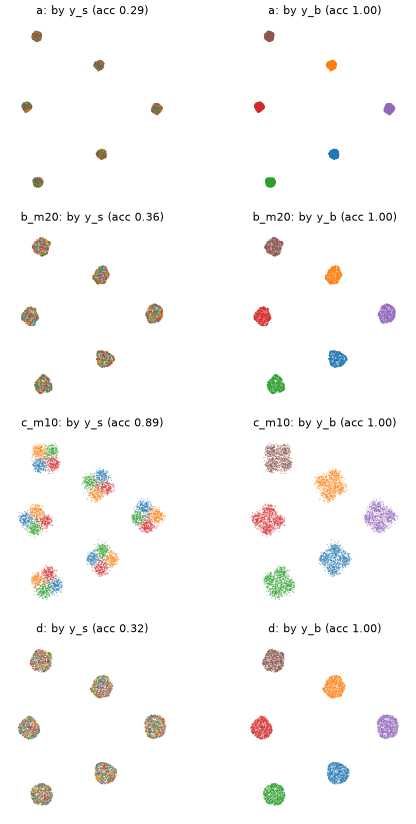
\includegraphics[height=0.45\textheight]{figures/additive_easy_seed0.png}
\caption{Orthogonal additive benchmark, selection seed 0. Left: colored by signal group. Right: colored by background cluster. Panel titles use internal run labels:
\texttt{a} = plain Neg-t-SNE; \texttt{b\_m20} = 20 uniform extra negatives per edge; \texttt{c\_m10} = 10 background negatives per edge (raw graph); \texttt{d} = spectrum reference. ``acc'' is kNN accuracy for the colored label. Background negatives split each background cluster into its four signal groups, but the six clusters stay apart (background accuracy 1.00).}
\label{fig:additive}
\end{figure}

\paragraph{Q2. When does global cPCA win?} Whenever the population identity holds and the signal lies mostly outside the background's high-variance directions.
\begin{itemize}
  \item \textbf{Additive benchmarks.} cPCA$\to$Neg-t-SNE reaches 0.980--0.989 (\cref{tab:additive}) and organizes the layout by signal across background clusters. Of a point's 15 embedding neighbors, a fraction of 0.805--0.820 share its signal group but come from a different background cluster, against 0.000--0.001 for background negatives \cdesc. It beats raw-graph background negatives by $+0.10$, $+0.40$ and $+0.11$ \cdesc.
  % source: results/phase5prep/cpca_summary.md
  \item \textbf{Interaction benchmark.} cPCA$\to$Neg-t-SNE also beats them: 0.984 vs 0.858, per seed $+0.086$ to $+0.155$ \cpre.
  % source: results/phase5a/tables_J.md
  \item \textbf{Selecting $\alpha$ without labels} was not a weak point. After embedding, the label-free $\alpha$ and the label-chosen $\alpha$ differed by at most 0.003 in mean signal accuracy \cdesc.
\end{itemize}

\paragraph{Q3. When do background negatives beat every global linear projection, and when does a local pipeline beat them?} \Cref{tab:subspace} summarizes.
% source: results/phase5b/tables_cyclic.md; tables_between.md; tables_cyclic_local_cpca.md; tables_between_local_cpca.md
\begin{itemize}
  \item \textbf{Cyclic benchmark.}
  \begin{itemize}
    \item Raw-graph background negatives beat the best cPCA variant, chosen per seed with labels over every $\alpha$ representative and $k \in \{3,5,10,20\}$, by $+0.36$ to $+0.41$ \cpre.
    \item They beat the best labeled block projection by $+0.29$ \cdesc.
    \item They reveal all six clusters (per-cluster accuracy $\ge 0.85$); the best projection reveals three (\cref{fig:cyclic}) \cdesc.
  \end{itemize}
  \item \textbf{Between-cluster benchmark.}
  \begin{itemize}
    \item The best cPCA variant (0.989) beats background negatives by 0.07--0.08 on every seed \cpre.
    \item Label-free cPCA fails (0.255), on both $\alpha$ and $k$ (\cref{sec:finding}) \cdesc: it picks $\alpha > 1$, which removes $U$, and its fixed $k = 10$ brings in $V$.
  \end{itemize}
  \item \textbf{Local cPCA}, added after the main results, with its predictions committed first. It runs k-means on $X_B$ (choosing $K$ by silhouette) and assigns each target to the nearest centroid. Within each cluster it runs cPCA at that cluster's label-free $\alpha$, then embeds the per-cluster coordinates with a large cluster offset so that no kNN edge crosses clusters.
  \begin{itemize}
    \item It found $K = 6$ with perfect agreement with the true clusters (adjusted Rand index 1.0) on every seed.
    \item It reached 0.984--0.992 on both benchmarks, at every $k \in \{3,5,10\}$, with label-free and true clusters alike. This confirmed the pre-registered predictions: at least 0.90, and label-free within 0.02 of true clusters \cpre.
    \item It beat background negatives on the cyclic benchmark by $+0.07$ to $+0.08$ on every seed \cpre.
    \item Discrete, well-separated background clusters are the most favorable case for it \cinterp.
  \end{itemize}
\end{itemize}

\begin{table}[htbp]
\centering
\small
\caption{Subspace-conflict benchmarks: within-cluster signal accuracy on confirmation seeds 3--5, mean [min, max]. ``Best'' rows are chosen per seed with labels (upper bounds). Local cPCA uses label-free clusters and $k = 3$; the other $k$ and the true-cluster versions are within 0.002 of it.}
\label{tab:subspace}
% source: results/phase5b/tables_cyclic.md; results/phase5b/tables_between.md; results/phase5b/tables_cyclic_local_cpca.md; results/phase5b/tables_between_local_cpca.md
\begin{tabular}{lcc}
  \toprule
  run & cyclic & between-cluster \\
  \midrule
  plain Neg-t-SNE & 0.334 [0.328, 0.344] & 0.349 [0.346, 0.352] \\
  uniform extra negatives ($m_B=40$) & 0.518 [0.503, 0.538] & 0.522 [0.516, 0.529] \\
  same-cluster oracle negatives ($m_B=80$) & 0.701 [0.689, 0.721] & 0.691 [0.684, 0.699] \\
  background negatives, raw graph ($m_B = 20$ / $10$) & 0.914 [0.912, 0.916] & 0.914 [0.910, 0.921] \\
  label-free cPCA$\to$Neg-t-SNE & 0.420 [0.377, 0.442] & 0.255 [0.244, 0.262] \\
  best cPCA variant (labels) & 0.530 [0.500, 0.551] & 0.989 [0.988, 0.992] \\
  best labeled linear projection & 0.624 [0.619, 0.628] & 0.989 [0.988, 0.991] \\
  local cPCA (label-free, $k=3$) & 0.989 [0.989, 0.990] & 0.987 [0.984, 0.991] \\
  \midrule
  detectability (high-D data) & 0.919--0.924 & 0.915--0.924 \\
  \bottomrule
\end{tabular}
\end{table}

\begin{figure}[htbp]
\centering
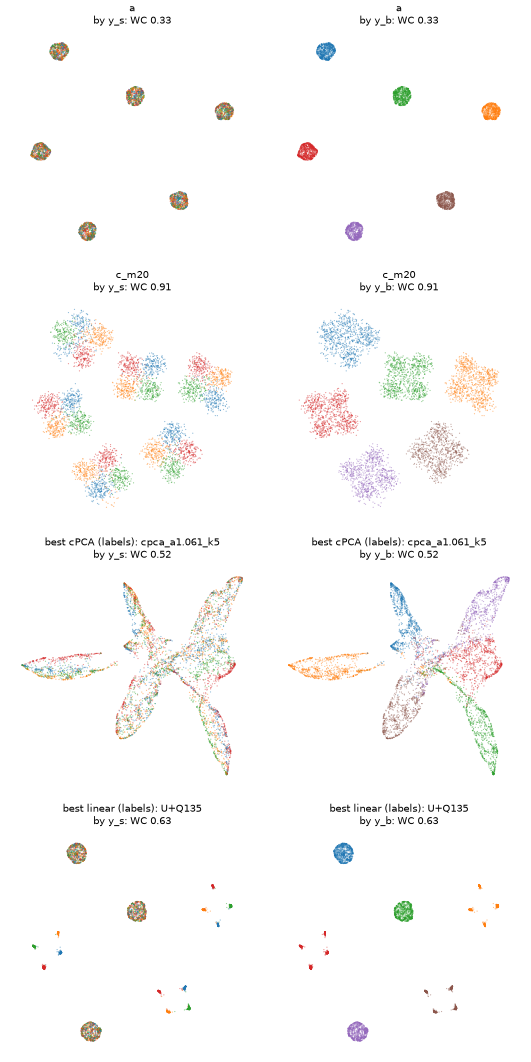
\includegraphics[height=0.6\textheight]{figures/cyclic_seed0.png}\hspace{2em}
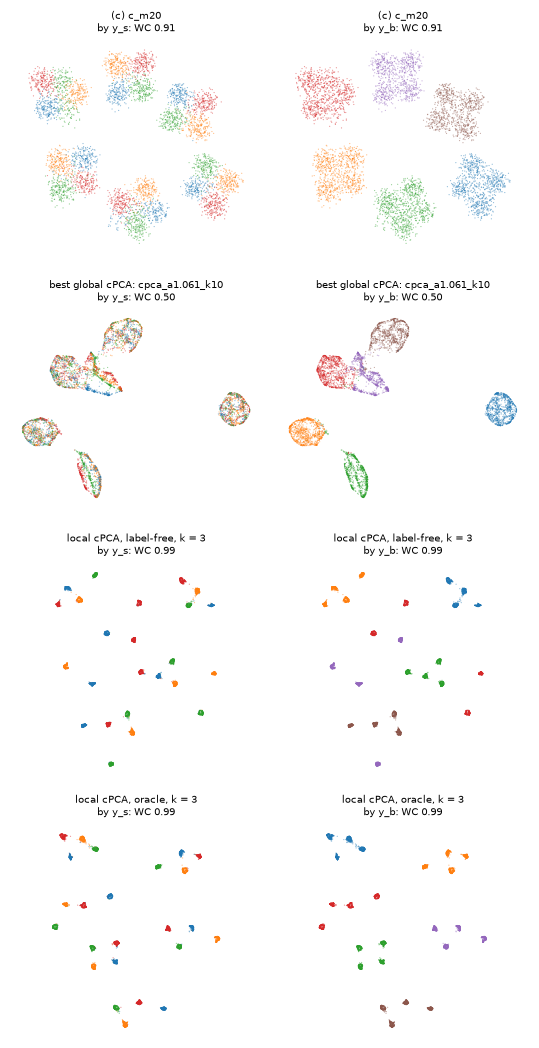
\includegraphics[height=0.6\textheight]{figures/cyclic_local_cpca_seed3.png}
\caption{Cyclic benchmark. In each pair of columns, the left panel is colored by signal group and the right by background cluster. ``WC'' is within-cluster signal accuracy.
\textbf{Left block (selection seed 0), top to bottom:} plain Neg-t-SNE (\texttt{a}); raw-graph background negatives with $m_B = 20$ (\texttt{c\_m20}), which split every cluster into its four signal groups; the best cPCA variant chosen with labels; and the best labeled block projection ($U$ plus blocks 1, 3, 5), which reveals only clusters 1, 3 and 5.
\textbf{Right block (confirmation seed 3), top to bottom:} raw-graph background negatives; the best global cPCA variant; local cPCA with label-free clusters; local cPCA with true clusters ($k = 3$). Local cPCA gives 24 tight islands, one per cluster and signal group. The islands of one background cluster are not placed together, because the cluster offsets make all clusters equidistant.}
\label{fig:cyclic}
\end{figure}

\subsection{Real data: MNIST-on-grass}
\label{sec:mnist}

\paragraph{The data} follow the construction of the cPCA paper \cite{abid2018cpca}.
\begin{itemize}
  \item MNIST digits 0 and 1 \cite{lecun1998mnist}, at 25\% intensity, are added to random $28\times 28$ grayscale patches cut from 1274 ImageNet grass photographs \cite{deng2009imagenet}.
  \item The target and background images are drawn from two disjoint halves of the photographs; the background is grass patches alone.
  \item Each seed has 5000 target and 5000 background images: selection seeds 0--2, confirmation seeds 3--5.
  \item The recipe follows the authors' notebook, with five documented deviations made for determinism and provenance.
\end{itemize}
The grass is added independently of the digit, so this dataset is additive (\cref{sec:identity}).

\paragraph{Pre-checks} \cdesc.
\begin{itemize}
  \item The digit signal is present in the raw kNN graph: digit kNN accuracy 0.90 on the raw images and 0.93 after PCA-50, against 1.00 on the clean digits.
  \item The raw graph's neighborhoods follow the grass: grass recall 0.44.
\end{itemize}
% source: results/mnist_grass/prechecks.md; results/bsgraph/phase1.md

\paragraph{Results} (\cref{tab:mnist,tab:mnist-cmp}, \cref{fig:mnist}).
\begin{itemize}
  \item \textbf{Raw-graph background negatives} ($m_B = 5$) beat t-SNE \cite{policar2024opentsne}, PCA-50$\to$t-SNE and plain Neg-t-SNE on every seed \cpre.
  \item \textbf{cPCA$\to$t-SNE} (label-free $\alpha$, 10 components) beats raw-graph background negatives on every seed \cpre.
  \item \textbf{Switching to the residual graph:}
  \begin{itemize}
    \item \BN{} beats raw-graph background negatives, t-SNE and PCA$\to$t-SNE on every seed \cpre;
    \item it ties cPCA$\to$t-SNE (not consistent) \cpre;
    \item it ties \methodname{} without background negatives (not consistent, with one exact tie) \cpre.
  \end{itemize}
  \item \textbf{Grass structure} \cdesc. Recall vs grass falls from 0.022 (raw graph) to 0.003, the same as cPCA$\to$t-SNE.
  \item \textbf{Checks.} The \BN{} seed-3 rerun was bit-identical. The raw-graph and t-SNE rows were reused from an earlier run, after checking that the code they depend on was unchanged and that every dataset matched its recorded checksum \cdesc.
\end{itemize}

\begin{table}[htbp]
\centering
\small
\caption{MNIST-on-grass, confirmation seeds 3--5: digit kNN accuracy (mean [min, max] and per seed) and recall vs grass (lower is better). No run was flagged.}
\label{tab:mnist}
% source: results/bsgraph/tables_phase2.md
\resizebox{\textwidth}{!}{\begin{tabular}{lccccc}
  \toprule
  run & digit acc. & seed 3 & seed 4 & seed 5 & recall vs grass \\
  \midrule
  \BN{} ($m_B = 1$) & 0.973 [0.972, 0.974] & 0.973 & 0.974 & 0.972 & 0.003 \\
  \methodname{} (no background negatives) & 0.972 [0.970, 0.974] & 0.971 & 0.974 & 0.970 & 0.004 \\
  raw graph + background negatives ($m_B = 5$) & 0.931 [0.926, 0.938] & 0.926 & 0.938 & 0.930 & 0.022 \\
  plain Neg-t-SNE (raw graph) & 0.858 [0.838, 0.871] & 0.838 & 0.871 & 0.866 & 0.079 \\
  t-SNE & 0.884 [0.872, 0.891] & 0.872 & 0.891 & 0.890 & 0.135 \\
  PCA-50$\to$t-SNE & 0.891 [0.883, 0.898] & 0.883 & 0.898 & 0.893 & 0.131 \\
  cPCA$\to$t-SNE & 0.955 [0.941, 0.979] & 0.941 & 0.979 & 0.943 & 0.003 \\
  \bottomrule
\end{tabular}}
\end{table}

\begin{table}[htbp]
\centering
\small
\caption{MNIST-on-grass pre-registered comparisons on digit kNN accuracy, confirmation seeds. Differences are first run minus second run.}
\label{tab:mnist-cmp}
% source: results/bsgraph/tables_phase2.md; results/mnist_grass/tables.md
\resizebox{\textwidth}{!}{\begin{tabular}{lccl}
  \toprule
  comparison & per-seed difference & mean & verdict \\
  \midrule
  \BN{} vs raw graph + BN & $+0.046, +0.036, +0.041$ & $+0.041$ & \BN{} better, consistent \\
  \BN{} vs cPCA$\to$t-SNE & $+0.032, -0.006, +0.028$ & $+0.018$ & not consistent \\
  \BN{} vs t-SNE & $+0.101, +0.083, +0.081$ & $+0.088$ & \BN{} better, consistent \\
  \BN{} vs PCA$\to$t-SNE & $+0.090, +0.076, +0.079$ & $+0.082$ & \BN{} better, consistent \\
  \BN{} vs \methodname{} & $+0.001, +0.000, +0.002$ & $+0.001$ & not consistent \\
  \midrule
  raw graph + BN vs t-SNE & $+0.054, +0.046, +0.040$ & $+0.047$ & raw graph + BN better, consistent \\
  raw graph + BN vs PCA$\to$t-SNE & $+0.043, +0.040, +0.038$ & $+0.040$ & raw graph + BN better, consistent \\
  raw graph + BN vs cPCA$\to$t-SNE & $-0.015, -0.042, -0.013$ & $-0.023$ & cPCA$\to$t-SNE better, consistent \\
  raw graph + BN vs plain Neg-t-SNE & $+0.088, +0.066, +0.065$ & $+0.073$ & raw graph + BN better, consistent \\
  \bottomrule
\end{tabular}}
\end{table}

\begin{figure}[htbp]
\centering
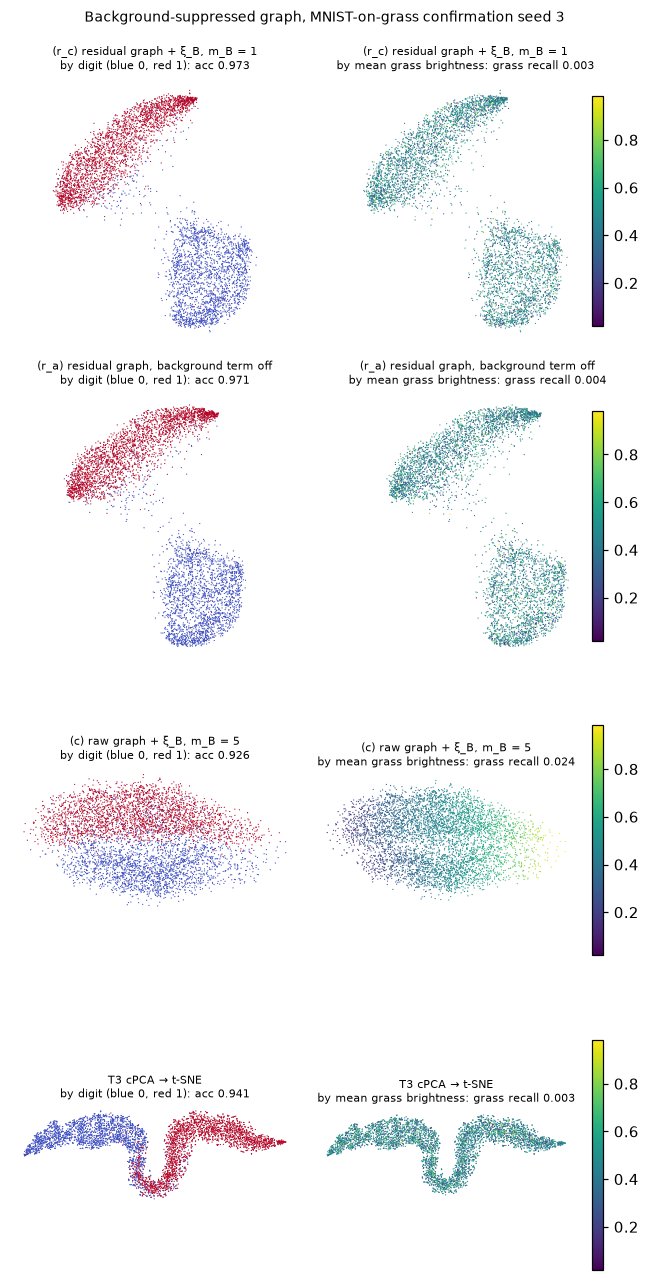
\includegraphics[height=0.55\textheight]{figures/mnist_residual_seed3.png}
\caption{MNIST-on-grass, confirmation seed 3. Left: colored by digit (blue 0, red 1). Right: colored by the mean brightness of each image's grass patch. Panel titles use internal labels, top to bottom: \texttt{(r\_c)} = \BN{}; \texttt{(r\_a)} = \methodname{} without background negatives; \texttt{(c)} = raw graph + background negatives; \texttt{T3} = cPCA$\to$t-SNE. On the residual graph the two digits form separate islands with no brightness gradient. On the raw graph the digits split within one blob that still runs from dark to bright grass.}
\label{fig:mnist}
\end{figure}

\clearpage
% =====================================================================
\section{What has and has not been tested}
\label{sec:gaps}

\begin{table}[ht]
\centering
\small
\caption{Every experiment, with its outcome for the method in the form tested. ``Raw'' means the raw kNN graph with background negatives; ``residual'' means \methodname{} / \BN{}.}
\label{tab:tested}
\begin{tabular}{p{2.9cm}p{2.4cm}p{1.2cm}p{3.6cm}p{4.2cm}}
  \toprule
  data & background & graph & competitors & outcome \\
  \midrule
  3 additive synthetic & additive, discrete clusters & raw & uniform, spectrum ref., (cPCA) & beats controls; cPCA better \\
  weak-signal stress sets & additive, signal weak in graph & raw & uniform, spectrum ref. & small gain on 2 of 3 levels \\
  interaction & signal depends on background & raw & cPCA, same-cluster oracle & cPCA better; beats oracle \\
  cluster-specific signal & cluster-specific signal maps & --- & cPCA & stopped: cPCA already solves it \\
  cyclic & subspace conflict & raw & cPCA, linear, oracle, local cPCA & beats all global linear; local cPCA better \\
  between-cluster & signal in between-cluster span & raw & cPCA, linear, oracle, local cPCA & best cPCA and local cPCA better \\
  MNIST-on-grass & real, additive & raw & t-SNE, PCA/cPCA$\to$t-SNE & beats t-SNE controls; cPCA better \\
  MNIST-on-grass & real, additive & residual & same, and raw & beats raw and t-SNE; ties cPCA \\
  \bottomrule
\end{tabular}
\end{table}

\paragraph{Gaps.}
\begin{enumerate}
  \item \textbf{Non-additive real data.} Every real-data result is on an additive dataset, where global cPCA is exact in population. This is also where the local residual graph's case against a global cPCA graph must be made (\cref{sec:dec-local}).
  \item \textbf{The residual graph on the subspace-conflict benchmarks.} These are the designs where global cPCA fails or needs labels. One question is whether the default $r = 2$ suffices against their 3-dimensional local nuisance (\cref{sec:residual-theory}).
  \item \textbf{Continuous or curved backgrounds.} Every background so far is made of discrete, well-separated clusters, which also favors cluster-then-cPCA pipelines.
  \item \textbf{The role of background negatives.} They are redundant on MNIST-on-grass with the residual graph, and untested with it elsewhere, for example when the residual graph is imperfect.
  \item \textbf{Label-free defaults beyond MNIST-on-grass.} $k_{\mathrm{loc}}$ and $r$ were checked on one dataset only.
  \item \textbf{The algorithm confound.} Comparisons with t-SNE-based controls also change the embedding algorithm. Without the background term, Neg-t-SNE was below t-SNE on MNIST-on-grass (\cref{sec:dec-neg}).
  \item \textbf{A single-stage schedule} has not been compared with the two-stage one.
  \item \textbf{Nonlinear contrastive methods}, e.g.\ contrastiveVI \cite{weinberger2023contrastivevi}, have not been compared.
  \item \textbf{Scaling.} Only $n = 5000$ has been tested. The residual construction does one small SVD per target point.
\end{enumerate}

% =====================================================================
\section{Proposed next steps}
\label{sec:next}

\begin{enumerate}
  \item \textbf{A real dataset with a non-additive background,} with \methodname{} (with or without background negatives) as the main method, against cPCA$\to$t-SNE, t-SNE and PCA$\to$t-SNE. The dataset is to be chosen together; it should be one where the nuisance interacts with the signal, so that global cPCA's identity fails.
  \item \textbf{Optional: the residual graph on the existing cyclic and between-cluster benchmarks,} against raw-graph background negatives and local cPCA. These benchmarks need no new data, and they test local versus global suppression directly.
  \item \textbf{What background negatives are for.} Test whether they help when the residual graph is imperfect, for example with a mis-sized $k_{\mathrm{loc}}$ or $r$. If they never help, drop them from the method.
\end{enumerate}

\bibliographystyle{plain}
\bibliography{refs}

% =====================================================================
\appendix

\section{Names used in this report}
\label{app:names}

The repository uses internal phase and run labels. This table maps them to the names used here. Paths are relative to the repository root.

\begin{center}
\small
\begin{tabular}{p{4.6cm}p{2.6cm}p{3cm}p{4.6cm}}
  \toprule
  name in this report & internal phase & internal label & results directory \\
  \midrule
  plain Neg-t-SNE & all & (a) & --- \\
  uniform extra negatives & 4, 5a, 5b & (b) & --- \\
  raw graph + background negatives & 4--MNIST & (c) & --- \\
  t-SNE-end spectrum reference & 4 & (d) & --- \\
  same-cluster oracle negatives & 5a, 5b & (o) & --- \\
  cPCA$\to$Neg-t-SNE / UMAP & 5 prep, 5a, 5b & (e2) / (e3) & --- \\
  t-SNE / PCA$\to$t-SNE / cPCA$\to$t-SNE & MNIST-on-grass & T1 / T2 / T3 & --- \\
  \methodname{} / \BN{} & bsgraph & (r\_a) / (r\_c) & \texttt{results/bsgraph/} \\
  \midrule
  additive benchmarks (orthogonal / overlapping / nonlinear) & 1, 4, 5 prep & easy / medium / hard & \texttt{results/phase4/}, \texttt{results/phase5prep/} \\
  weak-signal stress sets & 4 & stress & \texttt{results/phase4/stress/} \\
  interaction benchmark & 5a & Design J (t60\_proj\_g2) & \texttt{results/phase5a/} \\
  cluster-specific-signal benchmark & 5a & Design K & \texttt{results/phase5a/} \\
  cyclic / between-cluster benchmarks & 5b & L-cyclic / L-between & \texttt{results/phase5b/} \\
  local cPCA & 5b (extension) & local\_labelfree / local\_oracle & \texttt{results/phase5b/} \\
  MNIST-on-grass, raw graph & MNIST-on-grass & --- & \texttt{results/mnist\_grass/} \\
  MNIST-on-grass, residual graph & bsgraph & Phase 1 (graph), Phase 2 (embeddings) & \texttt{results/bsgraph/} \\
  \midrule
  within-cluster signal accuracy & 5a, 5b & WC & --- \\
  background-neighbor negative distribution & 2 & $\xi_B$ & \texttt{results/phase2/} \\
  \bottomrule
\end{tabular}
\end{center}

\section{Reproducibility}
\label{app:repro}

\paragraph{Code.} \url{https://github.com/Cassiebastress/bg-contrastive-ne} (public). Every result file records its software environment and the commit it ran at.

\paragraph{Pre-registration commits.} Each was made before the results it governs.
\begin{center}
\small
\begin{tabular}{ll}
  \toprule
  experiment & commit \\
  \midrule
  additive benchmarks: protocol and decision rules & \texttt{dad1c09} \\
  global metrics and thresholds, before any cPCA result & \texttt{23459ff} \\
  interaction / cluster-specific benchmarks: predictions; pre-registration & \texttt{4336ea0}; \texttt{9ed1110} \\
  cyclic / between-cluster: predictions; pre-registration & \texttt{04a1450}; \texttt{9c35a0b} \\
  local cPCA predictions & \texttt{a791d9b} \\
  MNIST-on-grass (raw graph): pre-registration; selection & \texttt{8f916ee}; \texttt{3dd613a} \\
  residual graph: graph-quality gate; embeddings & \texttt{3f0fc27}; \texttt{42bd31c} \\
  \bottomrule
\end{tabular}
\end{center}

\paragraph{Environment.}
\begin{itemize}
  \item Python 3.12, PyTorch 2.14.1 (CPU), numpy 2.5.2, scipy 1.18.1, scikit-learn 1.9.1.
  \item \texttt{contrastive-ne} v0.4.0 (upstream commit \texttt{d5f0b53}), vendored with an 11-line hook.
  \item openTSNE 1.0.4 \cite{policar2024opentsne}, used for the t-SNE controls.
\end{itemize}

\paragraph{Platforms.}
\begin{itemize}
  \item Synthetic experiments: an Apple M3 laptop, 4 threads.
  \item MNIST-on-grass: the McGill Mathematics Slurm cluster, AMD EPYC 9474F, CPU only, 1 thread per run, 24 runs in parallel.
  \item Before use, the cluster was validated: two runs were bit-identical, and the cluster differed from the laptop by at most 0.027 in within-cluster accuracy on a benchmark rerun.
\end{itemize}

\paragraph{Determinism.}
\begin{itemize}
  \item Deterministic PyTorch algorithms, fixed thread counts and seeded generators.
  \item Exact kNN graphs.
  \item A bit-identical rerun was checked in every experiment.
\end{itemize}

\section{Additional tables and figures}
\label{app:tables}

\begin{table}[ht]
\centering
\small
\caption{Residual-graph grid on MNIST-on-grass, selection seeds 0--2, mean [min, max]. Selected: $k_{\mathrm{loc}} = 30$, $r = 2$. The rule was the highest mean; variants within 0.002 counted as tied and went to the smaller $r$, then the smaller $k_{\mathrm{loc}}$. Edge purity is the share of graph edges joining same-digit images.}
\label{tab:grid}
% source: results/bsgraph/phase1.md
\resizebox{\textwidth}{!}{\begin{tabular}{lcccc}
  \toprule
  graph & graph digit acc. & edge purity & grass recall & clean-digit recall \\
  \midrule
  $k_{\mathrm{loc}}=15$, $r=0$ & 0.960 [0.959, 0.961] & 0.945 [0.943, 0.945] & 0.084 [0.083, 0.084] & 0.062 [0.060, 0.063] \\
  $k_{\mathrm{loc}}=15$, $r=1$ & 0.959 [0.958, 0.960] & 0.948 [0.947, 0.950] & 0.066 [0.065, 0.068] & 0.064 [0.061, 0.066] \\
  $k_{\mathrm{loc}}=15$, $r=2$ & 0.961 [0.959, 0.962] & 0.950 [0.949, 0.951] & 0.057 [0.054, 0.059] & 0.065 [0.063, 0.067] \\
  $k_{\mathrm{loc}}=15$, $r=5$ & 0.961 [0.958, 0.962] & 0.951 [0.950, 0.954] & 0.049 [0.047, 0.051] & 0.068 [0.065, 0.070] \\
  $k_{\mathrm{loc}}=15$, $r=10$ & 0.958 [0.955, 0.961] & 0.951 [0.949, 0.952] & 0.046 [0.045, 0.049] & 0.068 [0.066, 0.071] \\
  $k_{\mathrm{loc}}=30$, $r=0$ & 0.959 [0.956, 0.961] & 0.941 [0.938, 0.942] & 0.096 [0.093, 0.098] & 0.060 [0.057, 0.062] \\
  $k_{\mathrm{loc}}=30$, $r=1$ & 0.960 [0.959, 0.962] & 0.946 [0.944, 0.947] & 0.073 [0.072, 0.073] & 0.063 [0.059, 0.065] \\
  $k_{\mathrm{loc}}=30$, $r=2$ & 0.962 [0.961, 0.963] & 0.950 [0.949, 0.951] & 0.056 [0.054, 0.058] & 0.066 [0.063, 0.068] \\
  $k_{\mathrm{loc}}=30$, $r=5$ & 0.961 [0.960, 0.962] & 0.953 [0.952, 0.954] & 0.046 [0.043, 0.049] & 0.070 [0.067, 0.073] \\
  $k_{\mathrm{loc}}=30$, $r=10$ & 0.958 [0.955, 0.960] & 0.951 [0.950, 0.954] & 0.045 [0.041, 0.049] & 0.071 [0.068, 0.074] \\
  $k_{\mathrm{loc}}=100$, $r=0$ & 0.954 [0.951, 0.955] & 0.930 [0.926, 0.931] & 0.125 [0.122, 0.130] & 0.054 [0.050, 0.056] \\
  $k_{\mathrm{loc}}=100$, $r=1$ & 0.958 [0.956, 0.960] & 0.937 [0.934, 0.939] & 0.097 [0.094, 0.101] & 0.057 [0.054, 0.060] \\
  $k_{\mathrm{loc}}=100$, $r=2$ & 0.963 [0.962, 0.964] & 0.948 [0.947, 0.950] & 0.061 [0.059, 0.064] & 0.065 [0.062, 0.068] \\
  $k_{\mathrm{loc}}=100$, $r=5$ & 0.964 [0.962, 0.965] & 0.957 [0.955, 0.958] & 0.043 [0.040, 0.047] & 0.074 [0.069, 0.076] \\
  $k_{\mathrm{loc}}=100$, $r=10$ & 0.959 [0.958, 0.959] & 0.954 [0.953, 0.956] & 0.044 [0.040, 0.047] & 0.075 [0.071, 0.079] \\
  \midrule
  raw pixels & 0.904 [0.903, 0.905] & 0.844 [0.837, 0.851] & 0.439 [0.432, 0.447] & 0.020 [0.019, 0.023] \\
  PCA-50 & 0.935 [0.932, 0.938] & 0.872 [0.867, 0.878] & 0.337 [0.328, 0.348] & 0.020 [0.019, 0.022] \\
  global cPCA-10 (descriptive) & 0.970 [0.947, 0.986] & 0.956 [0.924, 0.978] & 0.006 [0.006, 0.006] & 0.065 [0.018, 0.103] \\
  \bottomrule
\end{tabular}}
\end{table}

\begin{table}[ht]
\centering
\small
\caption{Selection of $m_B$ on MNIST-on-grass, selection seeds 0--2: digit kNN accuracy, mean [min, max]. The rule was the highest mean, with ties going to the smaller $m_B$.}
\label{tab:mb}
% source: results/bsgraph/tables_phase2.md (appendix); results/mnist_grass/tables.md (appendix)
\begin{tabular}{lcc}
  \toprule
  $m_B$ & residual graph (\BN{}) & raw graph + background negatives \\
  \midrule
  0 & 0.972 [0.971, 0.974] & 0.850 [0.818, 0.876] \\
  1 & \textbf{0.973} [0.971, 0.974] & 0.923 [0.910, 0.931] \\
  2 & 0.972 [0.971, 0.973] & 0.935 [0.934, 0.936] \\
  5 & 0.972 [0.969, 0.974] & \textbf{0.937} [0.936, 0.939] \\
  10 & 0.970 [0.968, 0.972] & 0.930 [0.928, 0.932] \\
  20 & 0.969 [0.967, 0.971] & 0.924 [0.919, 0.927] \\
  40 & 0.968 [0.966, 0.969] & 0.922 [0.919, 0.925] \\
  \bottomrule
\end{tabular}
\end{table}

\begin{table}[ht]
\centering
\small
\caption{Additive benchmarks: pre-registered per-seed differences in signal kNN accuracy, background negatives minus control, confirmation seeds. All are consistent across 3 paired seeds \cpre.}
\label{tab:additive-cmp}
% source: results/phase4/tables.md
\begin{tabular}{lccc}
  \toprule
  control & orthogonal & overlapping & nonlinear \\
  \midrule
  plain Neg-t-SNE & $+0.589, +0.589, +0.568$ & $+0.227, +0.197, +0.218$ & $+0.504, +0.552, +0.507$ \\
  uniform, same $m_B$ & $+0.543, +0.538, +0.541$ & $+0.181, +0.169, +0.182$ & $+0.472, +0.492, +0.464$ \\
  uniform, best $m_B$ (20) & $+0.519, +0.489, +0.513$ & $+0.181, +0.169, +0.182$ & $+0.444, +0.439, +0.436$ \\
  spectrum reference & $+0.556, +0.547, +0.541$ & $+0.206, +0.198, +0.189$ & $+0.479, +0.508, +0.474$ \\
  \bottomrule
\end{tabular}
\end{table}

\begin{figure}[ht]
\centering
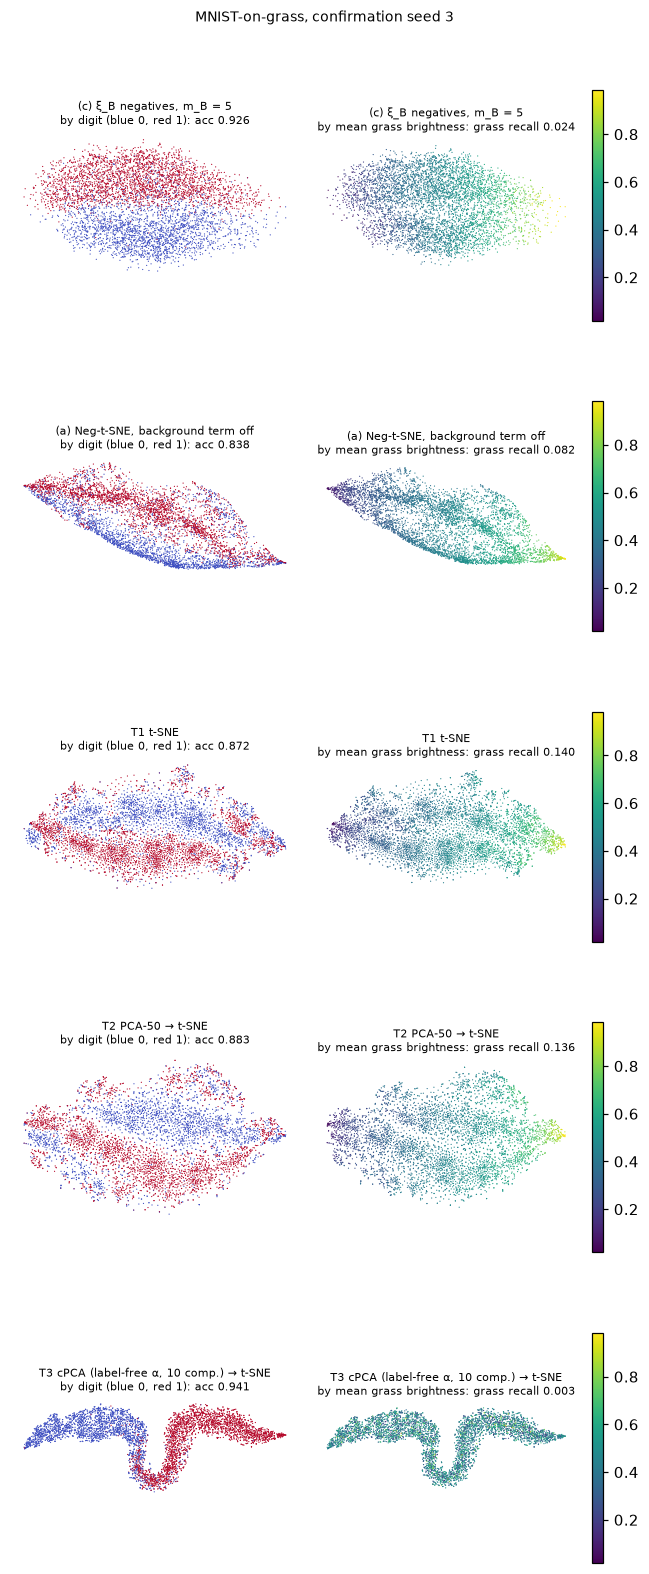
\includegraphics[height=0.75\textheight]{figures/mnist_controls_seed3.png}
\caption{MNIST-on-grass controls, confirmation seed 3. Left: colored by digit. Right: colored by grass brightness. Rows, top to bottom: raw graph + background negatives; plain Neg-t-SNE; t-SNE; PCA-50$\to$t-SNE; cPCA$\to$t-SNE. Plain Neg-t-SNE, t-SNE and PCA$\to$t-SNE are organized partly by grass brightness, and their bright-grass end mixes the two digits.}
\label{fig:mnist-controls}
\end{figure}

\end{document}
